
\rhead{Create Spotting}

\chapter{Create Spotting}
\label{sec:create_spotting}

\begin{figure}[!h]
\centering
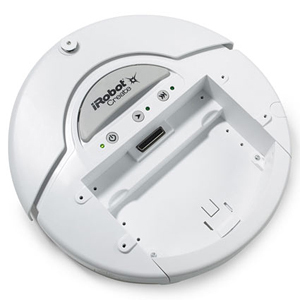
\includegraphics[width=0.8\columnwidth]{figures/4_create.jpg}
\end{figure}

\newpage

The previous chapters have explained the steps necessary to get a
robot platform, computer and associated components connected,
installed and ready to begin using.  However, the assignment
introduced in this chapter will not rely on much of that
infrastructure, so students can begin working even before the
development framework is assembled, tested and ready.  The purpose of
the Create Spotting assignment is for students to become familiar with
the Create hardware functionality and to highlight the importance of
scientific writing.  They need only access to a Create robot platform
as it comes out of the box.

% At the end of this chapter you will be able to:
% \begin{itemize}
% \end{itemize}

\section{Introduction}

One of the first things roboticists learn, perhaps to their dismay, is
that programming and using robots is \emph{not} like most other
programming and software development.  Software engineers can
sometimes get away with thinking of their computers as pristine
environments.  Programs do exactly what they are told to do, and if a
program fails to perform as expected, the error invariably arises
because the programmer failed to express the task correctly in code.
Finding the bug may not be trivial, but fixing it will make the
problem disappear.

Even in strictly digital environments, of course, this is a simplistic
view.  Users can act stupidly, maliciously or perversely.  Networks
can behave badly.  Data can become corrupt.  Major chip manufacturers
may introduce errors into their floating-point logic.  Even so, these
sources of chaos can be minimized with good, defensive programming
practice.

Not so with robots!  Robots, by their very nature, force computers and
programmers out of their comfortable, orderly digital environment and
into the noisy, messy, unpredictable, dangerous real world.  Much as a
general quickly learns that no battle plan survives contact with the
enemy, a roboticist soon finds out that no algorithm, even if it works
perfectly in tests and simulations, emerges unscathed from its first
attempt to sense and move and interact with reality.

Because of this fact, to a far greater degree than many other
disciplines within computer science, robotics is \emph{empirical}
and \emph{experimental}.  As such, a roboticist must learn the basic
tools of experimental science: how to observe behavior, design
experiments, record data, analyze results and report their
significance.  Throughout the course, students will develop these
skills, and they begin with an empirical investigation into the
behavior of an unknown robot.

% \begin{wrapfigure}{r}{0.35\columnwidth}
% 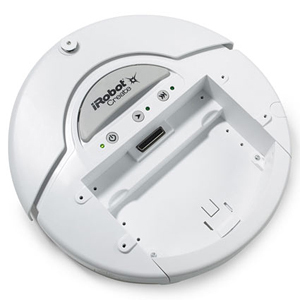
\includegraphics[width=0.32\columnwidth]{figures/4_create.jpg}
% \end{wrapfigure}

Assignment 0 is a written analysis of the built-in demos provided on the iRobot Creates.  This assignment is designed to:\\
\begin{itemize}
\item Get students acquainted with the iRobot Create hardware and to investigate the sensors and actuators used to control the Create's behavior.
\item Familiarize students with the scientific method, which is the basis for quantitatively acquiring new information.
\item Expose the students to the inherently unpredictable and nondeterministic nature of autonomous robotics.
\end{itemize}

Students should choose 2 of the 10 pre-programmed iRobot Create routines from the provided in the \href{http://www.irobot.com/filelibrary/create/Create\%20Manual_Final.pdf}{iRobot Create manual}. This assignment requires students to:\\
\begin{itemize}
\item State a testable hypothesis that can be validated quantitatively with statistical significance.
\item Design experiments to test the pre-defined demos that are reproducible in results.
\item Run multiple experiments to collect quantitative metrics; control variables used to gauge the validity/invalidity of the thesis should vary among experiments.
\item Analyze the results to determine the validity or invalidity of the hypothesis based on measurable evidence.
\end{itemize}

We would like to highlight that the students should not rely entirely on the descriptions provided by the demos as they are not always exhaustive. For example, some routines will react to obstacles or IR walls even though it is not mentioned in their description. For reference, the sensors are: IR receiver (detects Virtual Walls and Homebase), cliff sensors and bumper sensors.

Note: This assignment is not limited to the Create/ASUS platform and can apply to any robot system.

\section{Key Concepts}

\subsection{Project Writeup Format}

Each writeup is meant to be a scientific report about your project, the methods underlying your work, and its basis in the science of robotics.  As such, the paper should follow the scientific method:  observation, hypothesis, experiment, analysis, and conclusion.  It should be objective and scientific in tone (avoid informal writing and use the first person sparingly).  The paper should have a {\bf central thesis} stating your claims about what was accomplished or questions answered. Everything in the report should contribute toward the validity or invalidity of the thesis.  The paper should include the following sections:

\begin{itemize} 
\item Introduction:  The introduction should briefly state the problem and why it is relevant, state the thesis, and give a brief overview of how the paper will validate/invalidate the thesis.

\item Approach:  The approach describes the technical details of your work.  This section includes the underlying design and methodology and relevant details of the technical components.  Save comments about future extensions and the quality of the results for the discussion section.  Code snippets are acceptable in this section, however, you should not copy your entire program into the report.  

\item Experiment and Results:  In this section you should present the specific criteria that was used to gauge how the project validates/invalidates your thesis.  Presenting the results from multiple runs of your system is strongly encouraged.  

\item Discussion:  This section includes analyses of challenges and problems encountered, the strengths and shortcomings of the project, and potential future extensions.  This section is also where you should discuss why you made certain decisions regarding the methods and implementation of your project.  For final projects, this section will also contain brief comparisons to existing work.  

\item Conclusion:  A brief (1 paragraph at most) summary of the central thesis, its validity/invalidity, and what was learned from the project.  

\end{itemize} 


\section{Project Infrastructure}

The only hardware components required for this assignment are the iRobot Create base and the iRobot Battery. The iRobot Create accessories that can be utilized for the demos are the Virtual Wall and the Self Charging Home Base. (Please refer to 2.1 Hardware Components for descriptions on these parts).

\section{Instructions}

To run the demos:
\begin{itemize}
\item Put a battery in an iRobot Create and press the power button. Wait for the power LED to stop flashing.
\item Select a demo by pressing the ``Advance'' button (the button with a double forward arrow). The Create beeps to indicate the selected demo number. One long, low beep is equal to five short, high beeps. 
\item Press the play button to run the currently selected demo. 
\item Stop the demo by pressing either the ``Play'' or ``Advance'' button.
\item (optional) The home base must be plugged into the power outlet to be detectable by the Create.
\item (optional) To use a virtual wall, press the power button on the virtual wall. The slider on top of the virtual wall should be set to the ``4'-7'" range and the virtual wall should be placed in proximity of the Create.
\end{itemize}

\section{Expected Outcomes and Reports}

The purpose of the project writeups is to familiarize students with a style of scientific writing and validating their work through experimentation and writing.  What can be expected from the writeups is most of the reports are not consistent with the \href{http://en.wikipedia.org/wiki/Scientific_method}{scientific method}, which is the basis for quantitatively acquiring new information.  Below are general comments we present to the class to help the students expectations for the writeups and how to improve their writing skills for the subsequent reports, which will be beneficial for any career in the computing. 

\begin{itemize}
\item Your report lacked a \textit{testable hypothesis} with a quantitative metric that evaluated (validated or invalidated) through measurable evidence. In other words, your hypothesis cannot be tested using qualitative descriptions or value judgments.  Individual trials should be evaluated using metrics such as time to completion, ``success" rate (do not forget to define success), or number of collisions. Aggregate results from multiple trials should also be stated using statistics such as mean and variance across trials.  Tables with aggregate results are especially valuable to readers of your report.

\item The \textit{conclusion} must tie into the original \textit{hypothesis} stated in the introduction.  Think of the conclusion as the introduction looking back on the experiment and summarizing what was learned.

\item \textit{Value judgements} should not be used. Avoid using terms such as ``it worked well", ``the problem is simple and straightforward", or ``the robot behaved intelligently" because these are qualitative descriptions and cannot be measured. In general, do not use vague or relative language to describe the properties of your work.  Avoid narrating over your own observations from the experiment; let your data do the talking.  Videos are nice and very helpful, but alone are not sufficient for quantitatively evaluating your core hypothesis.

\item \textit{Reproducible description} of the methods employed.  We do not expect excessive detail or verbosity.  However, it is expected that any capable upper-level CS student should be able to reproduce your results from the description in the writeup.

\item \textit{Compositional organization}. The writeup should be properly sectioned into: Introduction, Approach, Experiment, Discussion and Conclusion. Specifically, the Introduction should state what you are testing and why it is important. The hypothesis must be clearly stated in the Introduction. The Experiment should state the metrics you will use to validate or invalidate your hypothesis. The Conclusion should be a summary of your central thesis, whether its valid or invalid based on what you measured in the Experiments section, and what was learned from the project. Secondly, we also expect basic compositional skills such as spelling, grammar and documentation organization. Additionally, illustrative and interesting visuals (pictures, illustrations and movies) and tables describing the trials/metrics help us quickly understand your methods and results.
\end{itemize}

\subsection{Grading Criteria}

The following outlines the grading criteria for this assignment. This is the same criteria used for the written portion of every assignment to follow:

\vspace{1cm}
\begin{tabular}{|l|l||l|l|}
\hline
{\large \bf Written Report} & \\
\hline
\hline
Introduction and Problem Statement & 7\% \\
$\rightarrow$ What is your problem? & \\
$\rightarrow$ Why is it interesting? & \\
\hline
Approach and Methods & 15\% \\
$\rightarrow$ What is your approach to the problem? & \\
$\rightarrow$ How did you implement your approach and algorithms? & \\
$\rightarrow$ Could someone reproduce your algorithms? & \\
\hline
Experiments and Results & 20\% \\
$\rightarrow$ How did you validate your methods? & \\
$\rightarrow$ Describe your variables, controls, and specific tests. & \\
$\rightarrow$ Could someone reproduce your results? & \\
\hline
Conclusion and Discussion & 8\% \\
$\rightarrow$ What conclusions can be reached about your problem and approach? & \\
$\rightarrow$ What are the strengths of your approach? & \\
$\rightarrow$ What are the shortcomings of your approach? & \\
\hline
\end{tabular}

\newpage
